\documentclass[11pt]{article}
\usepackage[letterpaper]{geometry}
\usepackage{microtype}
\usepackage{url}
\usepackage{setspace}
\usepackage{enumitem}
\usepackage{amsmath}
\usepackage{graphicx}
\usepackage{color}
\usepackage[dvipsnames]{xcolor}
\usepackage{soul}
\usepackage{hyperref}
\usepackage[numbers,sort&compress]{natbib}

% Hogg issues
\setlength{\topmargin}{0in}
\setlength{\headsep}{0in}
\setlength{\headheight}{0in}
\setlength{\oddsidemargin}{0in}
\setlength{\textheight}{9in}
\setlength{\textwidth}{6.5in}
\sloppy\sloppypar\raggedbottom\frenchspacing
\setstretch{1.08} % 
\renewcommand{\Large}{\normalsize} 
\renewcommand{\large}{\normalsize} 
\renewcommand{\paragraph}[1]{\medskip\par\noindent\textbf{#1~---}}
\setlist{topsep=0.75ex, itemsep=0.75ex, parsep=0ex} % This tightens up ALL lists.

\newcommand{\kw}[1]{{\color{RoyalBlue}[KW: #1 ]}}
\newcommand{\hogg}[1]{{\color{red}[Hogg say: #1 ]}}
\newcommand{\remove}[1]{{\color{red}\st{#1}}}
\frenchspacing


%TODO
%HOGG: put words on bias-variance

\begin{document}

\section*{\raggedright Mathematically principled machine learning approaches to ocean dynamics}

The theory of the oceans and the atmosphere is, fundamentally, a computational theory, which requires simulations to solve and understand their complex evolution.
These simulations are extremely expensive multi-physics, multi-scale computations, and yet they don't currently have anything like the resolution they would need to resolve all scales of physical interest.
At the same time, making predictions for weather and climate depends on being able to run very large numbers of these simulations, both to match the data in the sense of a digital twin for the Earth, and also to quantify uncertainties.

For all these reasons, the ocean dynamics community has been looking at machine learning (ML) approaches.
Emulators---ML regressions trained on good, first-principles, physics simulations---can predict the outcomes of physics simulations with far less computation than that used by the simulations on which they are trained.
Also, sub-grid models built out of ML components can be trained to predict the differences between low-resolution and high-resolution simulations, which arise from non-linear dynamics.
These can be used to either speed high-resolution simulations (by patching low-resolution simulations), or else to make predictions for small scales that aren't even resolved with the highest resolution simulations (that is, provide closure).

Generalizing beyond Earth science, there is a growing interest in replacing or augmenting solvers for partial differential equations (PDEs) with ML regressions trained on computed data.
These projects have applications across many physics and engineering domains.
Since PDEs are the underlying technology in simulations of physical systems at many scales from electronics to the entire visible Universe,
these approaches to speeding up PDEs will speed up any kinds of digital twins---virtual representations of objects or systems (in this case the ocean)---designed to reflect particular physical objects accurately.

Recent applications of emulation in ocean dynamics contexts have shown some important successes, for example
an idealized model for multi-decadal timescales based on neural operators \cite{bire2023ocean}, a regional emulation on subseasonal timescales 
\cite{chattopadhyay2023oceannet}, and a 3D global emulation on 30-day timescales
\cite{xiong2023ai}.
Recent work by PI Zanna builds ML-based ocean emulators for multi-century rollouts that incorporate atmospheric data~\cite{subel2024building}. 

These ML approaches are very promising; they are driving innovation and research in ocean science and PDEs.
Because of the immense computational speed-ups that they enable, they are making possible computational programs that weren't previously possible.
At the same time, PIs Hogg and Villar have warned that the introduction of ML in these contexts can lead to important statistical biases \cite{goodorbad}.
The important question is: How can we trust and verify predictions made by ML models trained on simulations?
A hallmark of contemporary ML methods---such as convolutional neural networks, and transformers---is that they are enormously over-parameterized, contain internal combinatorially large degeneracies, and are essentially impossible to interpret at the parameter level.
In addition and relatedly, ML models are generically subject to successful adversarial attacks.
These attacks are often very highly tuned, specific problems with specific trained models.
But they reveal that the ML models are not doing what we expect, and that they are uninterpretable, and (in some sense) untrustworthy.

The trustworthiness issue originates from the fact that the accuracy of a ML solution does not have guarantees at run time, which is particularly important when ML is being applied to problems that have inherently low risk tolerance, such as medical operations, self-driving cars, and studies of global climate.
The possibility of potential catastrophic failures casts doubt on adopting ML solutions at scale, especially in the domains of greatest interest to agencies (such as ONR) and researchers.
Thus some of the research proposed here has implications that go far beyond PDEs.

The question in this proposal is:
How can we make ML methods used to emulate or improve numerical solutions to PDEs---and in particular, in ocean dynamics---more trustworthy?
We will explore answers to this question in part by implementing exact symmetries and by forcing latent models to obey exact, local conservation laws (allowing for the fact that real data sets often break these symmetries), and in part by developing adversarial training strategies.
In this work, we are building on our research in mathematical machine learning, in which we have shown that making ML methods obey the exact symmetries of classical physics improves prediction accuracy for physics problems, permits out-of-sample generalization, and reduces training-set data requirements.
Here we propose to extend this work to ocean contexts, and to the specific cases of closure of PDEs and emulation.
And we propose to empirically test our successes with uncertainty quantification and adversarial attacks.

\kw{We should mention we will produce a suite of ML simulations that is robust}

\section{\raggedright Thrust 1: Learning ocean dynamics with the exact symmetries of classical physics.}

In this project, our aim is to use the power of ML to obtain fast and robust predictions of ocean dynamics, and to understand the mathematical properties of the proposed models. In this task, we focus on defining the ML models. We consider three settings (1) the more theoretical setting in which one needs to emulate the dynamics of a known partial differential equation and/or closures need to be resolved, (2) the more practical setting in which the governing equation of the dynamics is not known but a time series of observations are provided, and (3) a hybrid setting in which data (observations) are combined with parametric partial differential equations.

What makes our approach different from others bringing ML approaches to ocean dynamics is that the models we propose here will be consistent with some of the symmetries of classical physics, which include the coordinate freedoms of rotation and translation, and the corresponding conservation laws.
Our preliminary results show that incorporating these constraints improves the robustness and generalization of the models. In the subsequent tasks we propose to empirically and mathematically evaluate these claims.

\paragraph{The closure problem}
In high-dimensional dynamical systems such as turbulent fluid dynamics and astrophysical plasmas, the physical process occurs on a wide range of spatio-temporal scales, and often processes on different scales will have their effect cascade to other scales. 
Therefore, in the ideal scenario, it is important to model all scales at the same time.
However, the computational cost usually increases geometrically with resolution, rapidly making good simulations prohibitively expensive.
For this reason, simulations are usually truncated at some scale.
This truncation inevitably loses small-scale information necessary to obtain accurate results, including even on much larger scales, because of these cascading effects.
The closure problem consists of building an effective model for the influence of the discarded degrees of freedom for all of the dynamics.

Solving the closure problem involves building and incorporating a subgrid model to compensate for missing modes.
Traditionally, there have been many attempts to use heuristic or empirical physical arguments to capture the effects of small and ``meso'' scales in the resolved flows \cite{thuburn2014cascades,jansen2014parameterizing, mana2014toward, zanna2017scale, bachman2017scale, pearson2017evaluation, bachman2018relationship, jansen2019toward, bachman2019gm, grooms2015numerical, berloff2018dynamically, juricke2020ocean}.
These models are often physically motivated and interpretable.
In recent years, ML methods have demonstrated promising results in capturing the subgrid physics with parameterized models with many parameters \cite{rasp2018deep, Bolton2019,maulik2019subgrid, beck2019deep, yuval2020stable, guan2022stable, beucler2021climate, shamekh2022implicit, wang2022non}.
Compared to physically-motivated models, ML methods have the advantage of flexibility to match complex functions.
However, this often comes at a cost of interpretability and controllability.

In particular, work by Bolton and Zanna \cite{Bolton2019} uses ML to learn forces that can correct the difference between the high-resolution model and the low-resolution model obtained after coarse-graining. These ML models are good at predicting the subgrid forcing, but they have poor performance when integrated over long periods of time. One hypothesis for this failure mode is the learned model does not respect some fundamental symmetries in the underlying physical system.

In this Thrust, we will develop equivariant ML models (i.e., ML models that are designed to respect symmetries) to learn the dynamics of an ocean model in order to understand whether adding symmetries to our model will improve its long-term stability.
We remark that some of the existing ML approaches do account for energy constraints \cite{guan2023learning} and physical invariances \cite{frezat2021physical, guan2023learning, pawar2023frame, Bolton2019} in general scenarios. Our goal is to further extend these ideas to incorporate other forms of coordinate freedom, specifically targeting oceanic dynamics. We propose to adapt the techniques from \cite{villar2021scalars} and \cite{xu2022pde} to implement a symmetry-preserving ML model for the 2-layer quasi-geostrophic (QG) ocean model implemented in \cite{pyqg}. We conjecture that incorporating symmetries and coordinate freedoms arising from physical law will improve the performance of the ML models, especially in terms of the long-term stability of the simulations.

Following \cite{pyqg}, the two-layer QG equations in Cartesian coordinates are
\begin{align} \label{eq.QG1}
    \partial_t q_m + \nabla\cdot (\mathbf u_m q_m) + \beta_m \partial_x \psi_m + U_m\partial_x q_m = -\delta_{m,2}r_{ek}\nabla^2\psi_m +ssd\circ q_m, \\
    q_m = \nabla^2\psi_m+(-1)^m\frac{f_0^2}{g'H_m}(\psi_1-\psi_2), \quad m\in\{1,2\}
    \label{eq.QG2}
\end{align}
where $x$ is the zonal coordinate (east-west) and y is the meridional coordinate (north-south); $m$ is the index of the fluid layer (1 for the upper layer and 2 for the lower layer); $q_m$ is a pseudo-scalar which represents the potential vorticity (it is invariant under rotations and it changes sign under reflections); $\psi_m$ is a pseudo-scalar known as the streamfunction, which allows us to compute the (vector) velocity as 
$\mathbf u_m=(u_m, v_m) = (-\partial_y\psi_m, \partial_x \psi_m)$; $U_m$ is the prescribed mean zonal flow (in the $x$ direction); $\beta_m = \beta + (-1)^{m+1} \frac{f_0^2}{g'H_m}(U_1-U_2)$ is the meridional gradient of potential vorticity due to differential rotation and prescribed mean flow; $r_{ek}$ is the bottom drag coefficient with the ocean floor (a scalar); $\delta_{m,2}$ is a Kronecker delta that we use to indicate that this term only shows up for the lower layer; $f_0$ is the reference Coriolis frequency (a scalar); $g'$ is the reduced gravity (also a scalar); $H_m$ is the fluid layer thickness; $\nabla = (\delta_x, \delta_y)$ is the horizontal gradient operator; $ssd$ is a small-scale dissipation function from the numerical scheme (see \cite{perezhogin2023generative}, Appendix A). 



The large eddy simulation approach from \cite{sagaut2005large} decomposes the variables $\mathbf u, q, \psi$ into the sum of resolved variables $\bar{\mathbf u}, \bar q, \bar \psi$ and subgrid components  $\mathbf u', q', \psi'$. The resolved variables correspond to the coarser observations of the original variables (namely, the convolution of the original variables with a Gaussian filter or similar), and the subgrid components are unknown. 

The governing equations for the filtered solutions are:
\begin{align}
    \partial_t \bar q_m + \nabla\cdot (\bar{\mathbf u}_m \bar q_m) + \beta_m \partial_x \bar \psi_m + U_m\partial_x \bar q_m = -\delta_{m,2}r_{ek}\nabla^2\bar \psi_m + S_m +ssd\circ \bar q_m, \\
    \bar q_m = \nabla^2\bar\psi_m+(-1)^m\frac{f_0^2}{g'H_m}(\bar \psi_1-\bar \psi_2), \quad m\in\{1,2\},
\end{align}
where $S_m$ is the additional (scalar) subgrid forcing produced by the unresolved eddies on the resolved scales:
\begin{equation}
    S_m = \nabla \cdot (\bar{\mathbf u}_m \bar q_m - \overline{\mathbf u_m q_m})
\end{equation}

The closure problem amounts to modeling $S_m$ such that the integration of the filtered solution in a coarse simulation matches the filtration of the solution of a higher-resolution simulation. In \cite{perezhogin2023generative} PI Zanna and collaborators use ML models to learn $S_m$ from simulated data at different resolutions. 

We propose that incorporating symmetries in the learning of the subgrid forcing will improve the learning by reducing the sample complexity and generalization error. In order to incorporate the symmetries we propose to use invariant-scalar-based models similar to the ones proposed by PIs Villar and Hogg \cite{villar2021scalars}. Similar ideas have already been applied to learning closures on different fluid dynamics PDEs in \cite{xu2022pde}.

In a nutshell, the idea is to parameterize $S_m$ as the divergence or a learned vector (or pseudo-vector) field. The vector field is parameterized as an $O(d)$-equivariant vector function with input vectors $v_1,\ldots, v_n$ and scalars $s_1,\ldots, s_k$ can be written as 
$$f(v_1,\ldots, v_n, s_1,\ldots, s_k) = \sum_{t=1}^n f_t([v_i^\top v_j]_{1\leq i \leq j \leq n },\ s_1, \ldots, s_k)v_t.$$
It may be needed to generalize this model to incorporate pseudo-vector and pseudo-scalar inputs and outputs. See \cite{gregory2023geometricimagenet} for a potential approach.

In this subtask we propose to:
(1) design an equivariant ML model to learn closures using techniques from \cite{villar2021scalars, xu2022pde}, (2) design a set of experiments to empirically assess the performance of the equivariant models in comparison with baseline ML models, (3) apply these ideas to simulated data from the ocean model QG equation, (4) provide a robust software package to reproduce these experiments and that can be extended to other equations.
See Section \ref{sec:deliverables} for more details on the deliverables on work plans. 

%This Thrust aims to improve oceanic simulations in two parallel direction: building ML-enhanced simulations and end-to-end emulation of simulations. On one hand, we will create end-to-end ML emulator to reduce the computational cost of creating large scale simulations. On the other hand, we will apply ML methods to replace uncertain terms in QG models in order to improve accuracy of existing model; 

\begin{figure}
    \centering
    \begin{minipage}{0.37\textwidth}
    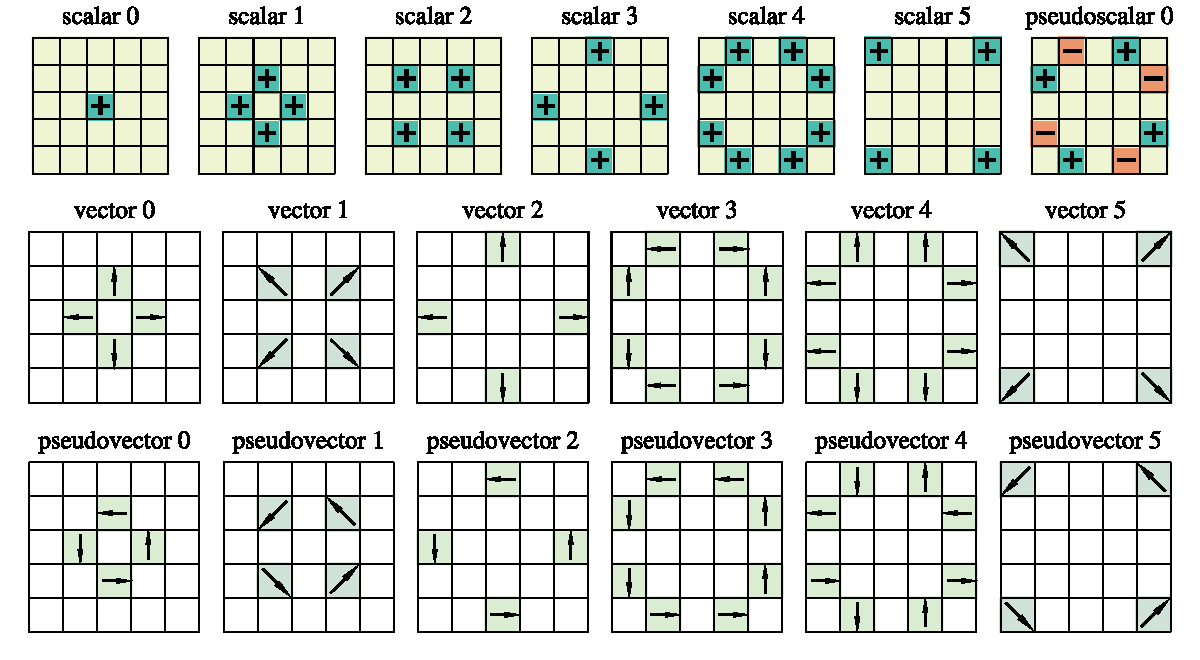
\includegraphics[width=\textwidth]{figures/filters_m5.pdf}
    \end{minipage}
    \begin{minipage}{0.62\textwidth}
    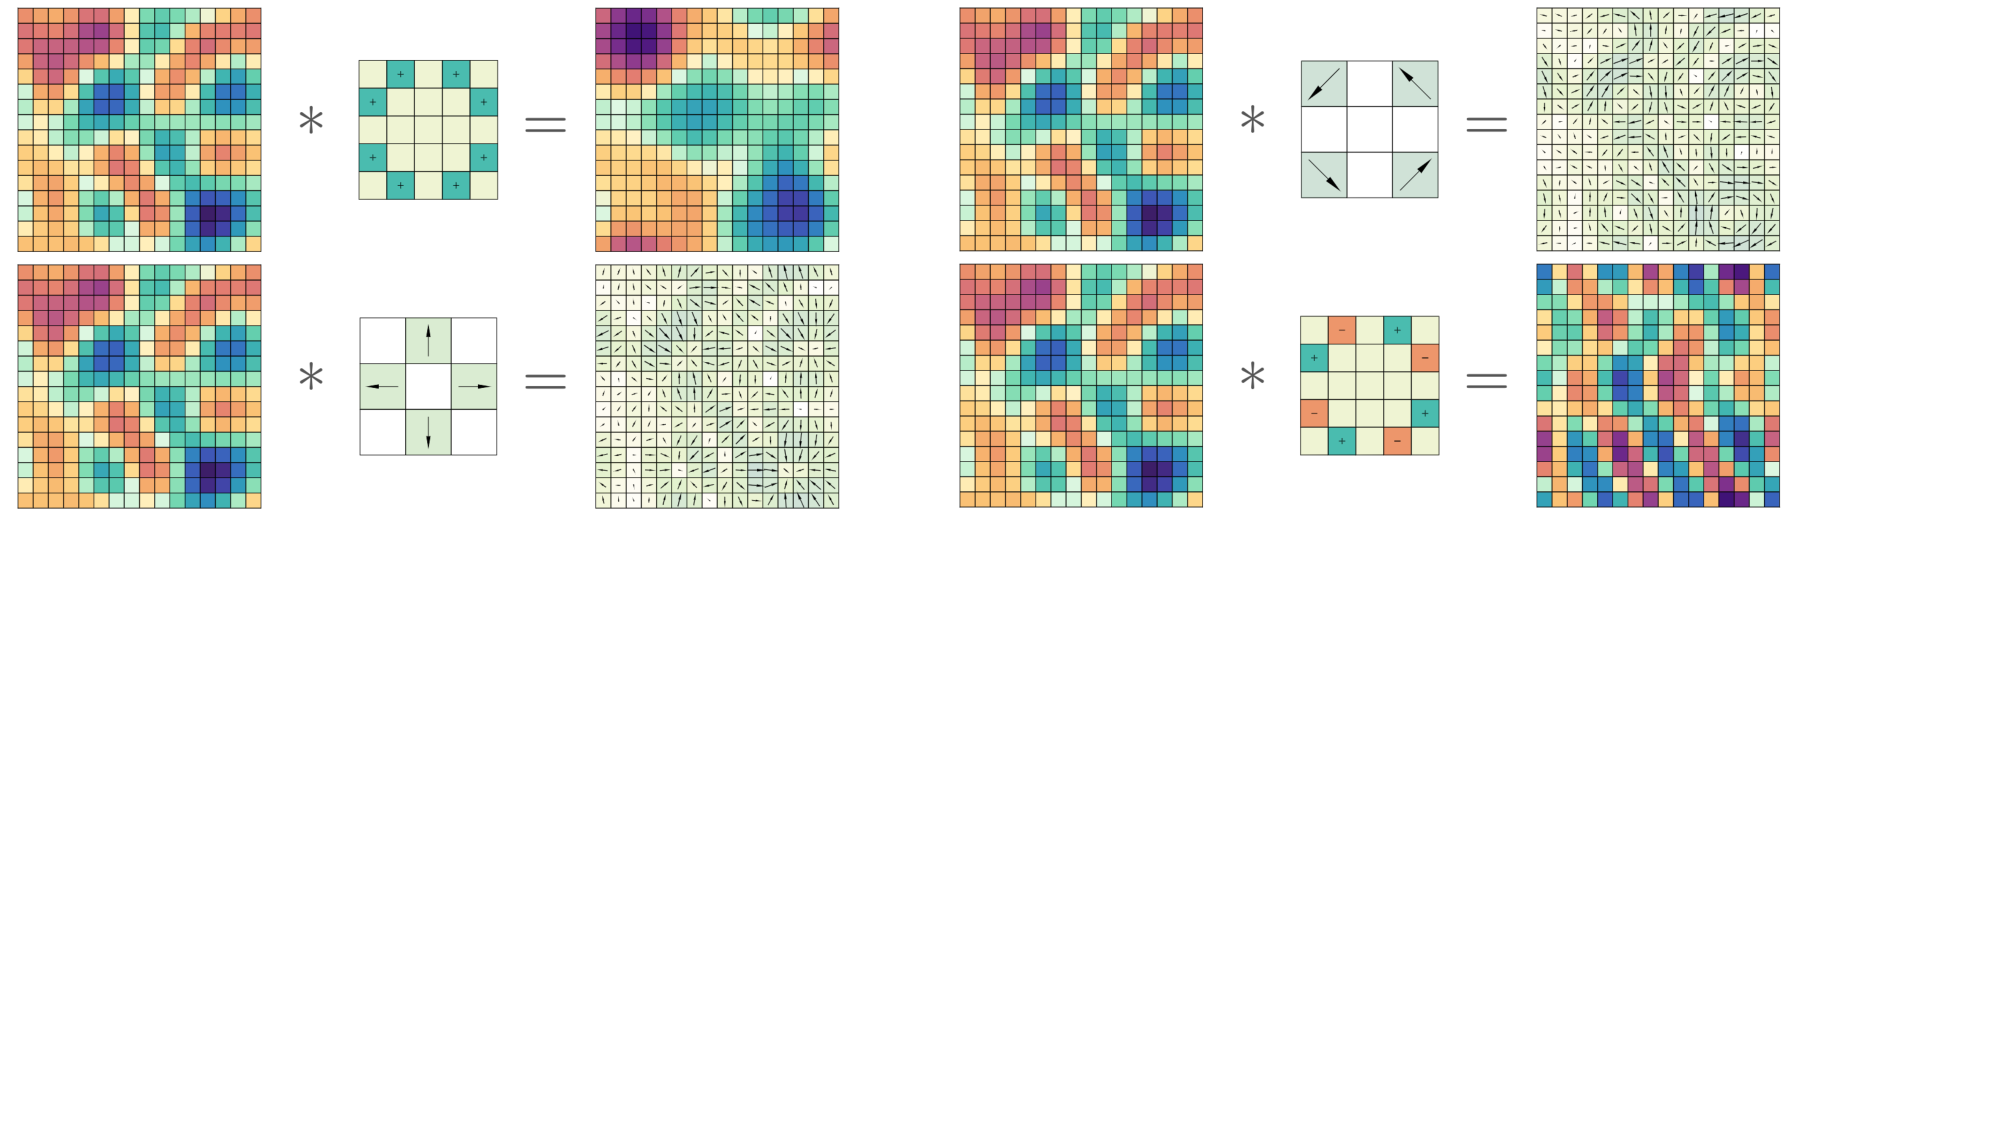
\includegraphics[width=\textwidth]{figures/convs.pdf}
    \end{minipage}
    \caption{(Left) The 5x5 scalar, pseudoscalar, vector, and pseudovector symmetric filters of GeometricImageNet for 2-D images. (Right) Convolution of a scalar image with different geometric filters. Note the convolution with a scalar filter can be seen as the discretization of a diffusion operator, and the convolution with the vector filter resembles a discretization of the gradient. In general any symmetric discretization of any coordinate-free operator (gradient, divergence, curl) could be expressed in terms of our symmetric filters.}
    \label{fig.GINet}
\end{figure}

\paragraph{End-to-end emulation of simulations}
\kw{We should probably be more precise about what ocean simulations we are going to deliver and how impactful they are.}
Ocean dynamics involves processes at many different scales. This means a detailed ocean simulation requires resolving small-scale processes over a large volume, which demands significant computational power.
Instead of solving the dynamic equations from first principles, a promising and increasingly popular way to amortize the computational cost is to train a ML model over a set of training simulations. Once the ML model is trained, one can use it to generalize to settings where the model is not trained. This method has shown promising results in a number of multiscale problems, including weather forecasting \cite{Pathak2022FourCastNetAG} and cosmological simulations \cite{CAMELS:2020cof}. However, existing methods often employ ML methods that do not explicitly preserve symmetries in the simulations, which could lead to potential inaccuracy. The goal of this task is to investigate whether equivariant ML models can outperform non-equivariant models for ocean modeling.

In \cite{Gregory2023EquivariantGC} we introduced GeometricImageNet, a equivariance-preserving counter part of the convolutional neural network (CNN). This model replaces the standard filters of the CNN with symmetric vector and tensor filters. These filters are convolved with vector and tensor images where the multiplication in the convolution is replaced by an outer product. This results in higher-order tensor layers that are subsequently composed with Einstein-summation contractions to reduce their order (see Figure \ref{fig.GINet}).  

Recently, in \cite{gregory2024robust} we use the GeometricImageNet model
to implement an emulator of the 2D compressible Navier-Stokes equation. Our result shows a significant improvement in accuracy and long-term stability when using an equivariant model over a non-equivariant model, as shown in \ref{fig:cfd_results}. This paper won a best paper award in the Machine Learning for the Physical Sciences workshop at NeurIPS 2024.

We propose to expand the effort we have done for Navier-Stokes to ocean models in this task. We are going to create a bank of reference simulations using the state-of-the-art codebase \kw{From Zanna}, then we are going to repeat the experiments we have done for the Navier-Stokes equations to see whether equivariant models show the same degree of improvement in accuracy for the now more sophisticated dynamical system. In this task, we expect to produce an emulator that can generate a large suite of simulations as well as understand whether equivariance is useful for modeling the ocean. The emulator produced in this task will also be useful as the foundation of Thrust 2 and 3.\kw{Briefly mention deliverables.}

\begin{figure}
    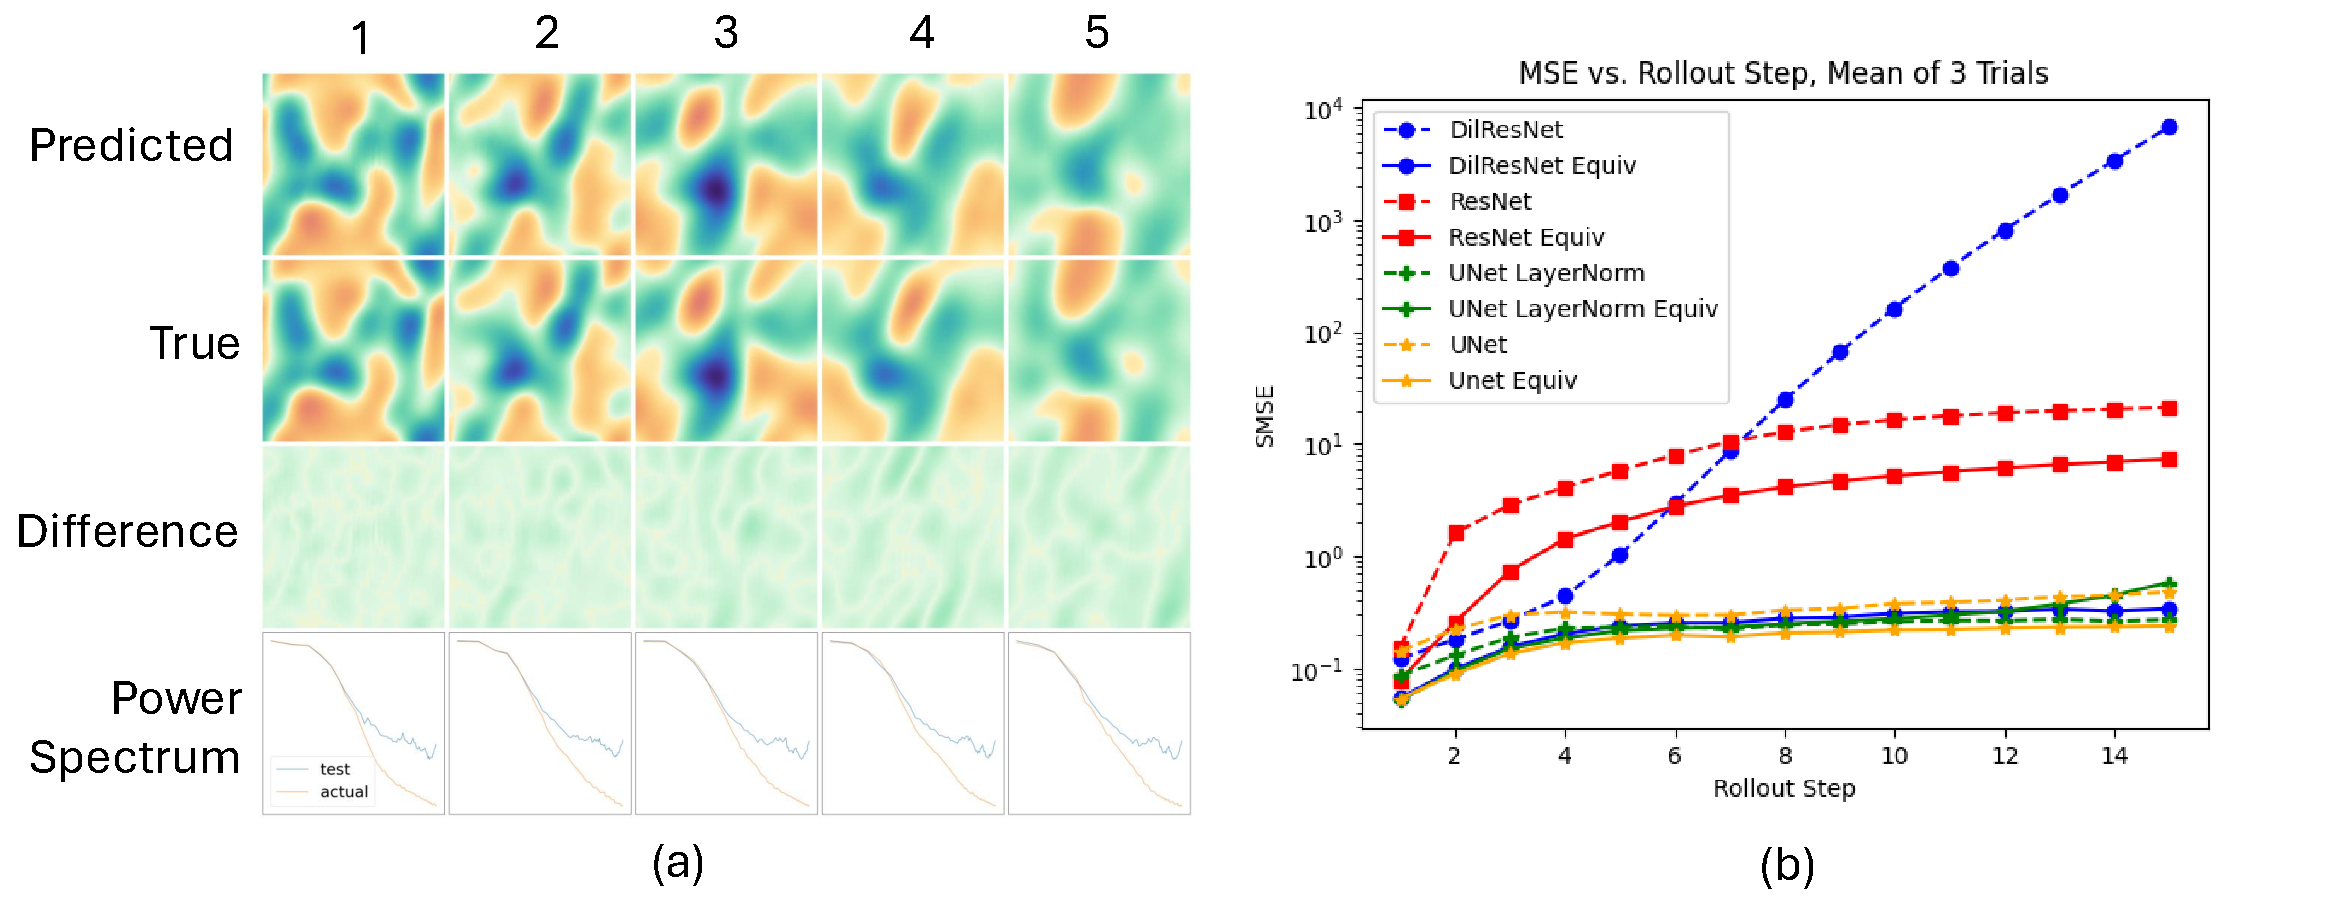
\includegraphics[width=\textwidth]{figures/cfd_results.pdf}
    \caption{(a) Five steps of rollout using the best performing model, the equivariant UNet without LayerNorm. 
    The x-component of the velocity is plotted.
    (b) Comparison of test performance over a 15 step rollout.
    The SMSE is shown for \textit{each} step, rather than a cumulative loss.}
    \label{fig:cfd_results}
\end{figure}


\paragraph{Hybrid method}
Although emulators can be useful for quickly creating large amounts of simulations and can be used in downstream tasks, such as comparing with real data, the accuracy of the simulations produced will be fundamentally limited by the accuracy of the simulation used to train the emulator. Therefore, improving the quality of the simulation tool kits we have is as important as speeding up the simulation process with emulation. ML methods offers tremendous flexibility to learn complicated function, but this flexibility can sometime limit the maximum accuracy of a model. Therefore, combining ML methods with traditional PDE solvers has been a popular way to model dynamical systems when there is a strong requirement on the accuracy of the simulation \cite{Kidger2022OnND, Rackauckas2020UniversalDE}.

Instead of learning an end-to-end emulator of the simulation, in this task we aims to improve the accuracy of the simulations by replacing certain terms in eq. \ref{eq.QG2} with ML models. One way this can be achieved is through fitting some of the more uncertain term to observational data.
As a proof-of-principle step, we are first going aim to recover certain specific terms used to generate the data with ML models, that is to first generate a set of reference simulations, then try to recover some terms we deliberately leave out in the QG equation with ML methods. This will test the identifiability of the PDE model from data in practice. For example, $r_{ek}$ is a coefficient which is often assumed to be a fixed value. Instead, we can leave that as a free parameters and try to fit it with data. This process can also be applied to other more complicated terms in the equation (though we are aware that the inverse problem is not always solvable). We are also going to benchmark whether equivariant model outperforms its non-equivariant counterpart in recovering the missing term. Once we have validated the performance of our pipeline with our own simulation suite, we are going to improve our hybrid model by calibrating it to publicly available data \cite{2004AGUFMSF31A0712O}. 
As a result, this task will deliver a framework of ML-enhanced simulations designed for modeling ocean dynamics, which can be fitted to real data to capture unknown physics while maintaining the structure in eq. \ref{eq.QG1} that are stemmed from physical principle, such that it is capable to robustly generalize to systems that are significantly different from existing simulations.



% \kw{Original Thrust 2}

% \paragraph{Emulators}
% In Thrust~1, we propose to learn closure terms that can be added to PDE solvers to account for sub-grid physics not tracked at the scale of the finite-resolution solution grid.
% These closure terms enter the equations or PDE solver like additional force terms.
% In principle, if they are learned accurately, the addition of these terms will improve the simulations.
% This is not guaranteed, however: Even if a function appears to do a good job of explaining the difference between the single-timestep force calculation in a low-resolution and the same, smoothed down to low resolution from a high-resolution force calculation, that does not guarantee that the addition of this term will improve the roll-out of many low-resolution time-steps of the PDE solver; small errors can amplify in the roll-outs.
% Indeed, when learned closures are used in PDE integrations, they often don't work very well \cite{perezhogin2023generative, Bolton2019}.

% One alternative to this approach is to perform emulations not just of a subgrid force term, but of the entire input--output relationship of the PDE solver.
% That is, learn an emulator function $f_{\Delta t}$ that takes as input the entire system state at time $t$ and delivers as output the entire system state at time $t+\Delta t$.
% If an accurate function can be learned, if that function can be evaluated quickly, and if the time interval $\Delta t$ can be made large, this emulator could be very valuable. This is the approach taken by neural operators from the physics-informed ML literature \cite{karniadakis2021physics}, which have been recently applied to ocean models \cite{bire2023ocean, chattopadhyay2023oceannet}.

% For training data in Thrust~2, our default plan is to use the GFDL CM2.6 simulations of ocean dynamics \cite{delworth2012simulated} and the filtering package \cite{loose2022gcm}, similar to \cite{subel2024building}.
% The simulation landscape is changing, so there might be alternatives to use instead, but for the purposes of this proposal---which is focused on mathematical methods---it isn't critical that we be at the absolute bleeding edge.
% One issue with emulating simulations of this type is that there is different time and spatial frequency structure in the evolution of different components; for example, temperature fields change on much different timescales than velocity fields.
% Recent work by Subel and Zanna \cite{subel2024building} has managed this by lowering time and spatial resolutions with sensible rebinnings of the simulation data; we would plan to work similarly.
% One difference between our simulation data and that work, however, is that \cite{subel2024building} concentrate on modeling temperature fields, which are scalar fields, and we are interested in exploiting the geometric structure and dynamical couplings of scalars, pseudo-scalars, and vectors (and tensors and pseudo-tensors derived therefrom), so we will build emulators not just for temperature, but also for velocity and potential vorticity.

% \paragraph{Equivariant ML for grids of vectors and tensors}
% The key idea underlying this thrust is that the PDEs in play are equivariant to a large number of physical symmetries, including translation, rotation, and reflection.
% In prior work, we have constructed a generalization of a convolutional neural network, the GeometricImageNet \cite{gregory2023geometricimagenet}, which takes advantage of the convolutional idea in ML, but implements also these geometric symmetries.
% This model is capable of representing scalar, vector, and tensor functions that are approximately equivariant to translations, rotations, and reflections.
% In detail, the GeometricImageNet model components are exactly equivariant to integer-pixel translations and 90-degree rotations (plus axis-aligned and diagonal reflections), and preserves the geometric structure of vectors and tensors.
% This model is ideally suited to emulation of mappings from scalar, vector and tensor image inputs to scalar, vector, and tensor outputs on a pixel grid.

% \paragraph{Emulation accuracy improvements from imposing symmetries}
% Our proposal is to train an emulator, with GeometricImageNet components.
% We will compare the outputs of the emulator to the output of full PDE solves,
% and emulators created for this problem previously \cite{subel2024building}.
% We will also compare our emulator to equivalents of the ``online'' experiments from Thrust~1, in which a low-resolution PDE solve is computed, with a learned closure term.

% The emulator involves a GeometricImageNet, and the GeometricImageNet, like all ML methods, involves a large number of investigator choices.
% These include choice of loss function, number of layers, and geometric properties of the latent variables at each layer.
% We propose to perform some reasonable investigation of these ``hyperparameter'' choices as we train different versions of the emulator.

% We conjecture that the accuracy of the emulator will depend strongly on the time interval $\Delta t$ over which the emulator is trained to make input--output predictions.
% Our goal will be to find time intervals $\Delta t$ over which the emulation is accurate, but far faster to execute than a full PDE solve.
% In this Thrust, accuracy will be assessed with the loss (the magnitude of the difference between the prediction and the true label (simulation) in the test set, but in the next Thrust, there will be a full uncertainty quantification.

% Because the dynamical system is nonlinear and technically chaotic, it is impossible for any simulation to remain accurate over long time intervals (longer than some Lyapunov time).
% Thus even the physical simulations are only accurate over some range of time intervals $\Delta t$.
% On longer time scales, there may be mean statistics of the ocean currents or kinetic energies that are more stably predicted than the precise velocity field (CITE SOMETHING).
% These kinds of predictions are harder to rigorously test, but ....

% Our main conjecture is that imposing symmetries---making the emulator equivariant to more groups---will make the emulator more accurate at fixed training-data size and model complexity than a CNN-based emulator that does not respect the rotation and reflection symmetries.
% We will test this by training matched GeometricImageNet and u-net [HOGG: MAYBE?] models (matched in terms of numbers of layers and [WHAT ELSE]) on [WHAT DATA?] and comparing predictions.
% Here in Thrust~2 this is a conjecture about the loss function, but in Thrust~3 (below), this will be elevated to a conjecture about uncertainty and susceptibility to adversarial attack.

% One limitation of many current ML methods working on the two-layer ocean model is that they are usually working on square grids.
% These grids are superimposed on a very complex ocean morphology, on the sphere (or near-sphere) that is the Earth.
% Thus the square grids have complications.
% Perhaps the primary complication is that different grid cells represent different ocean volumes (grid cells nearer to coordinate poles are smaller than grid cells farther).
% A stretch goal of this research is to include metric information into the GeometricImageNet model, appropriate at each grid point to the local coordinate metric.
% Because GeometricImageNet manages scalar, vector, and tensor fields, it can manage this tensor field, which is a fixed field on the grid.
% It is an interesting side project to see if introduction of the coordinate metric field into a GeometricImageNet model improves predictive accuracy.

% Deliverables: Results, a paper, public toy problem setups for the ML community, PhD student and undergraduate research training.

\section{\raggedright Thrust 2: Toward modeling real data with symmetry breaking}

\kw{Add features real life data has and study them, expect to characterize bias and come up with a theory}

\kw{Need to mod the following paragraph}
While Thrust 1 focuses on improving and speeding up simulations in an ideal situation, the focus of Thrust 2 will be on handling data that are not exactly equivariant. While the underlying physical phenomenons in the real world such as ocean currents obey physical laws and therefore are exactly equivariant, the process of capturing or collecting data related to these physical phenomenons often breaks the exact equivariance. One example of this is taking an image of the ocean, which introduces discretization to the underlying continuous physical phenomenon. Another example is when we fail to model relevant quantities and vector fields, and removing them from the model breaks the symmetry (see \cite{villar2023passive}). 

In addition to discretization and modeling issues, it is inevitable for real life measurements to be contaminated by noise, which do not follow the same equivariance structure the interested process has. This means our data is not exactly equivariant, but instead contains signals that are exactly equivariant. In the simplest case, this process of taking data from an equivariant process can be defined as $\mathbf{d} = f(\mathbf{s}) + \mathbf{n}$, where $\mathbf{d}$ is the vector of data we obtain, $\mathbf{s}$ is the process that is equivariant, $f$ is a function that operates on $\mathbf{s}$ that could break the equivariance, e.g., discretization, and $\mathbf{n}$ is the random noise that is not equivariant.
Once the non-equivariant effects are introduced in the data, the data is no longer exactly equivariant but approximately equivariant.
The main questions that this Thrust aims to address can then be phrased as: given some data $\mathbf{d}$ that contains a signal that follows a particular equivariant structure, can we develop a method to extract the equivariant component from the data? Ultimately, we will not be able to perfectly extract the exactly equivariant signal from the approximately equivariant data, as that would require perfect characterization of the noise. So instead, the next best objective that is achievable is to bound the bias induced by the noise as much as possible. 

As the community begins to realize the importance of understanding approximate equivariance in order to apply equivariant models to real data, there have been some preliminary results in the literature \cite{Wang2022ApproximatelyEN, huang2021traffic}. For instance, in \cite{huang2024approximately} we mathematically study the bias-variance trade-offs of reducing the amounts of symmetries that a model implements. 
In this Thrust, we build on top of the infrastructure prepared in Thrust 1, but shift our focus to adding effects to understand the behavior of equivariance models when presented approximately equivariant data. This Thrust contains two complementary directions  

\paragraph{Understanding the scale of equivariant signals}
In the example from \cite{gregory2024robust} illustrated in Figure \ref{fig:cfd_results} we used a GeometricImageNet which is an architecture similar to convolutional neural network (CNN) but with imposed equivariance to emulate simulations of 2D compressible Naiver-Stokes equation. Once we trained the network in a supervised setting, we also inspected how the network would perform in ``roll-outs", i.e. integrating the trajectories from an initial condition using the network as a forward step. This is usually a good measure of whether the training is robustly capturing the physics or just overfitting to the data.

One of the major surprises we found in this study was that by introducing dilation to a ResNet architecture \cite{yu2017dilated}, that is, by introducing gaps between elements in the convolution kernels, we improved the rollout accuracy by a factor of $\sim 20$ while reducing the number of parameters by a factor of 2. On the other hand, we repeated the experiment with the corresponding non-equivariant baselines, and the results of the dilated ResNet were catastrophic: it was three orders of magnitude worse than the non-dilated version. This result suggests that the equivariant neural networks can pick up signals from specific scales, hence drastically improving the generalization accuracy. In many analyses related to physics systems, the accuracy of analysis often peaks when the scale of tools matches the scale of the data \cite{}\kw{I am pretty sure there are some Fourier analysis classic examples here}. 

In this task, we aim to mathematically and empirically analyze the joint effects of equivariance and scale.
We are going to investigate the role scale plays in training an equivariant neural network and aim to come up with a concrete formalization of the response of equivariant neural network to data as a function of scale under discretization. Ideas of this sort have previously appeared in the numerical analysis literature, showing that numerical methods based on discretizations that respect the symmetries of the underlying problems outperform ones that do not \cite{verstappen2003symmetry}.  The empirical study will be done with training data from the 2-layer QG ocean model as described in eq\ref{eq.QG1}, for which we have control over the scales of features. The next step is to train a collection of equivariant neural networks on the generated data, while varying the scale of the kernel used in the network, to investigate the dependence of the kernel size on the equivariant scale.. 


\paragraph{Disentangling equivariant processes from noise}

\kw{Good to have some references about SOTA in literature}
\cite{Wang2022ApproximatelyEN}
Another difference between theoretical data and real data is the presence of noise. Since noise is not expected to be equivariant, adding noise to any equivariant signal will break the symmetry. Noise could originate from multiple types of sources at different scales. To illustrate this, let's use taking a satellite picture of the ocean as an example: at the pixel scale, there will be instrument noise from the camera that introduce fluctuation in the pixel reading; at the largest scale, there will be processes that irrelevant to the objectives such as cloud occlusion. 

The concrete definition of the problem in this task is: Given some noisy observation of a process that exhibits some equivariance, can we disentangle the information related to the equivariant process from the noise in an unsupervised manner?

As a starting step, we will use the simulations generated in Thrust 1 as the base, then we are going to add different realizations of noise to the simulations to create signals that are not exactly equivariant.  We will repeat the experiment in task 1, except now we introduce a simple yet controllable Gaussian noise process following a specific power spectrum. In this way, we can control whether the noise is more prominent in smaller scales or larger scales. 




\section{\raggedright Thrust 3: Adversarial attack and robustness of equivariant neural network}
% Reference: Perezhogin et al \url{https://arxiv.org/pdf/2302.07984.pdf}
\kw{The main deliverable here is how emulator can break and how do we prevent them from breaking.}

\kw{Worst case scenario attack: Can we create small perturbation to induce catastrophic failure. Mention Dilated ResNet in Wilson paper.}

While Thrust 2 investigates how bias is introduced steadily via noise, this Thrust looks into how bias can be introduced so drastically that it creates catastrophic failures, and how to defend against such catastrophic failures.
When simulating a particular PDE, errors accumulate as we integrate forward in time.
Traditional PDE solvers have guarantees on how rapidly the error can grow, often related to the order of the solver. For example, the Euler method has global error that grows linearly.  However, there are no such guarantees for ML based methods. Most of the uncertainty quantification approaches are based on estimating the bias and the variance of the predictions via bayesian approaches or other machine learning models \cite{perezhogin2023generative}.

%As we mentioned in Thrust 2, this lack of guarantee is not only  unsettling from a rigor point of review, the practical reason to avoid using methods without such guarantee is to avoid potential catastrophic failures.
As we have shown in \cite{gregory2024robust}, catastrophic failures did occur when using a dilated ResNet to model a compressible Navier-Stokes equation. Another form of catastrophic failures these models may be susceptible to are adversarial attacks.


Adversarial attacks are an interesting phenomenon that was identified in large machine learning models \cite{goodfellow2014explaining} about ten years ago. In many  highly-accurate machine learning models, a small, carefully crafted,  perturbation to the input data can drastically change the output of the method. One of the classic examples of an adversarial attack is the single-pixel attack \cite{su2019one}, in which one only needs to change the value of one-pixel of the input image to alter the result of a classification task.

In the context of ocean simulations, the question of interest is whether similar small perturbation can lead to a drastic deviation from a physical model. This is especially important when rolling out a learned emulator to an ocean model, since noise can accumulate and interact with the simulation non-linearly.


Compared to standard ML methods, equivariant models have more constraints in their architecture. It is possible that at least certain kinds of attacks are likely to be less effective or not effective at all.  There exists some literature on adversarial attacks of equivariant models \cite{schuchardt2023provable}, but similar to approximate equivariant models, the literature in adversarial attacks in the context of equivariant model is still underdeveloped. 

In this Thrust, we will explore how to empirically avoid catastrophic failures when applying ML methods to ocean simulations in two steps: First we will create experiments to adversarially attack equivariant models. The goal of this task is to understand the adversarial robustness of the proposed models empirically. The second step in this Thrust is to build methods that are robust against such attacks, possibly following ideas from \cite{schuchardt2023provable}.

%\paragraph{Creating the attack}

% It would be nice if we can create some ocean example
%There are two main directions in creating adversarial attacks: white-box attacks and black-box attacks. White-box attacks means we have access to the internal of the models such as gradient at the intermediate steps within a model to construct an attack.
%Black-box attack is the opposite of a white-box attack, meaning we can only rely on the input and output of the models to construct the adversarial attack. This is a more challenging task \cite{Papernot2016PracticalBA}
%Based on the work in Thrust 1 and Thrust 2, both the simulations and ML models we are investigating will be automatically differentiable, which enables the possibility of creating white box attacks.

%\paragraph{Defending the attack}

% How to we defend against failure? Basically list all the failure model, and see what are the things we can add to our model or project our model to make it more robust.



% \paragraph{Uncertainty quantification}

% In general, in all areas of PDE solving and forward simulation of physical systems, uncertainty quantification (UQ) is challenging.
% The uncertainty in a prediction is expected to be strongly dependent on the physical state of the system, and (in the case of roll-outs), the timespan of the PDE integration.
% It is also difficult to verify or validate any uncertainty quantification, since the state of the system is high dimensional:
% It is hard to span all of the physical states that might affect the uncertainty.

% At the same time, UQ is essential to any scientific program.
% This is especially true for ocean physics, which is critical for climate studies, where scientific uncertainties are of enormous importance for planning and policy.

% Classical methods for uncertainty quantification involve injecting low-amplitude noise into initial conditions and comparing the final-state predictions, with and without noise injected.
% There are different methods here, of different levels of sophistication (CITE THINGS).

% \paragraph{Generative models for UQ}
% In the last few years, ML regressions have been augmented or replaced by generative models, in which the ML method learns a generator that can generate samples from a non-trivial distribution that is learned from input data.
% In detail, in a generative model, the ML method learns a probability distribution function (pdf; or a function proportional to the pdf) from data, in such a way that the method can draw samples from that pdf.
% The objective is to make the training data high probability under the learned pdf, and for sampling from the learned pdf to be computationally efficient.
% Recently it has been shown that generative models are effective for UQ in ocean contexts [CITE ZANNA].

% Importantly for our purposes, we are interested in generative models that can generate data examples conditioned on input features.
% For example, in Thrust~1, the goal is to learn closure terms for a PDE solver, in which the training data consist of lower and higher resolution data from the same integration.
% A generative solution to this problem permits sampling from the distribution of all possible differences or all possible closure terms that might be in play, conditioned on the lower-resolution data.
% In general there is such a distribution, since there are multiple high-resolution states can be consistent with the same low-resolution state.
% In the limit that the pdfs are correctly learned, samples from the conditional distribution span the uncertainty, such that the variance (and skew and so on) of the sampling distribution represents the variance (and skew and so on) of the uncertainty on the prediction.
% That is, a generative model naturally produces the relevant UQ.

% From this perspective, the leading generative methods at the present day are variational autoencoders (VAEs), generative adversarial networks (GANs), normalizing flows, and diffusion.
% Each of these have different strengths and weaknesses.
% Recently GZ and PZFG (CITES HERE) have applied VAE and GAN subgrid-forcing models to obtain simultaneously more accurate low-resolution simulations and also associated uncertainties.
% They find that generative ML models perform better than ML regressions for subgrid forcing, and, at the same time, deliver reasonable uncertainty estimates.

% Our proposal is to reimplement VAEs for UQ on the closure problem, following GZ, PZFG (CITES), but with the enforced exact symmetries of Thrusts~1 and 2.
% We also propose to, for the first time in PDE contexts, train a diffusion model to do the same thing, as a comparison for the VAE.
% Diffusion is a method in which a neural network is trained to learn a forcing term in a stochastic differential equation such that fair samples of data (closure terms, in our case) can be generated by running forward a differential equation starting at noise initial conditions.
% SOLE: HOGG CAN WRITE MATH HERE; HE KIND-OF UNDERSTANDS IT NOW.

% \paragraph{Generalization benefits from symmetries}
% The main goal of Thrust~3 is to develop generative-model-based approaches to UQ, in the context of enforcing the exact symmetries of classical physics.
% Once that is in place, however, it opens up new questions.
% For example: Does adding new symmetries to ocean dynamics simulations reduce uncertainty?
% That is, does the restriction of the function spaces to those that respect exact equivariances to rotation, reflection, and translation (say) also reduce the variance of the prediction pdfs?
% We conjecture that the answer will be in the affirmative: Introduction of appropriate inductive biases should reduce model capacity but increase model accuracy.
% It is part of this proposal to test this conjecture.

% In support of this conjecture, ... 
% SOLE: YOU could put something here about Teresa's result that introducing symmetries might reduce variance.
% In general we need a discussion here of rigorous results relevant to the above conjecture.

% SOLE: We could think about whether we could also make a conjecture about the bias. HOGG thinks we can, because there are results about generalization when equivariance is imposed, right?

% Stretch goal: We can implement a diffusion model as a new kind of generative model to compare with the VAE and GAN models.
% Diffusion is a new, successful generative ML model, based on stochastic processes.
% It is very promising for applications of this kind, in which a probability distribution (the distribution of predicted closures or emulated final states) lives in a very high dimensional space (the space of all reasonable initial conditions).
% We propose to develop an equivariant conditional diffusion model and compare it to the VAE and GAN

% HOGG: Deliverables for the UQ part.

% \paragraph{Adversarial attacks and UQ}
% Although these generative-model approaches to uncertainty quantification are good approaches, we expect that they will, in the end, under-estimate the uncertainty associated with the emulators.
% One reason for this is that all expressive ML models are subject to adversarial attacks [CITE].
% In astrophysics, it has been shown that adversarial attacks are successful against most methods in use [CITE]; on very general grounds we don't expect the situation to be different for ocean dynamics.
% Thus it makes sense to adversarially attack ocean dynamics emulators and ask whether it is possible to design attacks that generate deviations of model predictions that are far larger than what's expected from the rsults of standard UQ methods.

% For our purposes here, an adversarial attack to an emulator would be a tiny change to the initial conditions of the emulator that produces a large and unphysical change to the output of the emulator.
% The input change is considered tiny if the amplitude is small enough such that the input given to the emulator represents a perfectly reasonable input, given the elements of the test set.
% The output change is considered large and unphysical if the output of the emulator departs substantially from the simulation (the physical model), when both the emulator and the simulation are started at the same initial conditions.
% Unfortunately, by construction in these problems, it is computationally expensive to verify that a change is unphysical; we return to this challenge below.

% Once we can find adversarial attacks against ocean emulators, two questions arise.
% The first question is: Are the UQ estimates substantially in error?
% On the one hand, adversarial attack vectors are likely to represent only a tiny fraction of any measure on the input space (initial conditions, say) of an emulator.
% On the other hand, successful adversarial attacks indicate that the emulator is not emulating precisely what is desired or required.
% Thus there is a real-world question about the significance of any successful adversarial attacks for assessing the veracity of a UQ analysis.

% The other question that arises is: Are equivariant models---or models that implement more symmetry groups---less susceptible to adversarial attacks than traditional models---or models that implement fewer groups?
% Our conjecture here is that more symmetric models should be subject to fewer or less severe attacks.
% This is because the model that is equivariant to more groups has less flexibility, and the flexibility that has been removed is flexibility that represents unphysical or physically incorrect modes or behaviors.
% At fixed training-data size, but comparable overall model complexity, the equivariant model should have fewer wrong behaviors, in some sense.

% \paragraph{Finding adversarial attacks affordably}
% As noted above, the verification of an adversarial attack is computationally expensive; how to proceed?
% If the simulations were inexpensive and differentiable (that is, if the derivative of the output with respect to input was computable), the attack could be discovered by moving the initial conditions in directions that maximize the discrepancy between the derivative of the emulator and the derivative of the simulation.
% This is not possible, and even running a few simulations to identify an attack is a significant cost.
% Thus we have to find the attacks by indirect means and then verify likely candidates.

% For some kinds of simulations, there are conservation laws in play.
% For example, in small-scale simulations of ocean subvolumes, there are exact conservation laws for momentum or salinity [CITE].
% For other kinds of simulations, there are mean statistics of ocean currents that are expected to be relatively stable or vary slowly with input parameters, for example WHAT [CITE].
% Since the emulators we build will be fully differentiable, for the emulators it is possible to follow directions of maximal derivatives in these conserved quantities or average statistics, starting from initial conditions that exist in the test set.
% The approach to attack discovery is to find small changes to the initial conditions that lead to very large changes in these conserved quantities or mean statistics; such a change would be an \emph{attack candidate}.
% Attack candidates can be verified as good attacks by running one additional simulation, at the perturbed initial conditions, and comparing it to the simulation run for the corresponding test-set element.

% Of course in nonlinear systems, there can be steep derivatives of output with respect to input.
% Thus we expect that not all attack candidates will verify as true attacks.
% In detail, the choice of conserved quantity or mean statistics will matter.
% The existence and discovery methodology for adversarial attacks in ocean contexts will be publishable in the ocean-science and ML literatures.

% Once good adversarial attacks are found, they can be compared with the UQ results:
% Do we find that we can adversarially generate emulation errors that are much larger than the UQ suggests?
% Furthermore, successful attacks on different models can be compared:
% Do we find that the success of attacks depends on the symmetries in play?

% HOGG: RETURN TO THE CONCEPT of trust that is in play at the beginning of this proposal.

% Deliverables: Paper on how to attack in a geophysics context.
% Paper on the susceptibility to attack of emulators with different equivariances, and implications for UQ and the believability of UQ analyses.
% Code.

\section{\raggedright Deliverables and Work plans} \label{sec:deliverables}

We will conduct the following research activities:
\begin{enumerate}
    \item We will generate a library of simulations for training using the open-source code \cite{pyqg} made available by Zanna's group. We will create a version with the full equations set and another version with the subgrid forcing term left out, such that we can establish a baseline of the discrepancies when the forcing term is completely omitted.
    \item We will train \textbf{non-symmetry-preserving} models along with the version of \textsc{pyqg} in which the subgrid forcing term is omitted. This should get close to the simulations using the full equations set but may have long-term stability issues.
    \item We will train \textbf{symmetry-preserving} models along with the version of \textsc{pyqg} in which the subgrid forcing term is omitted. We anticipate this model is going to outperform the non-symmetry-preserving model.
    \item We will compare the functional behavior of the learned subgrid term in both ML models, and construct a theory on the difference in performance between a symmetry-preserving model and a non-symmetry-preserving model in the context of the closure problem.
\end{enumerate}

Given the proposed activities, we anticipate the following deliverables from this Thrust:
\begin{enumerate}
    \item A theoretical understanding on what role symmetry plays in modeling complex physical system with ML, specifically when used together with a physics-driven model.
    \item The library of simulations generated will be made available to the public. This provides the community with a domain-specific benchmark dataset.
    \item Our code will be open-source, and the tightly integrated machine-learning--physical model can be a blueprint for other researchers to build on top of.
    \item Machine learning models for emulation of ocean dynamics and closures that are equivariant and robust to adversarial attacks. 
    \item Activities such as curating a well-put-together library can create a lot of research opportunities for junior researchers such as undergraduate and graduate research assistants. On one hand, the domain-specific knowledge from Zanna's group hones the student's understanding of the physical model. On the other hand, the students are also exposed to state-of-the-art ML applications. This project will help train next-generation scientists specialized in ocean dynamics who are well-versed in both physical modeling and ML.
\end{enumerate}


\begin{figure}
    \centering
    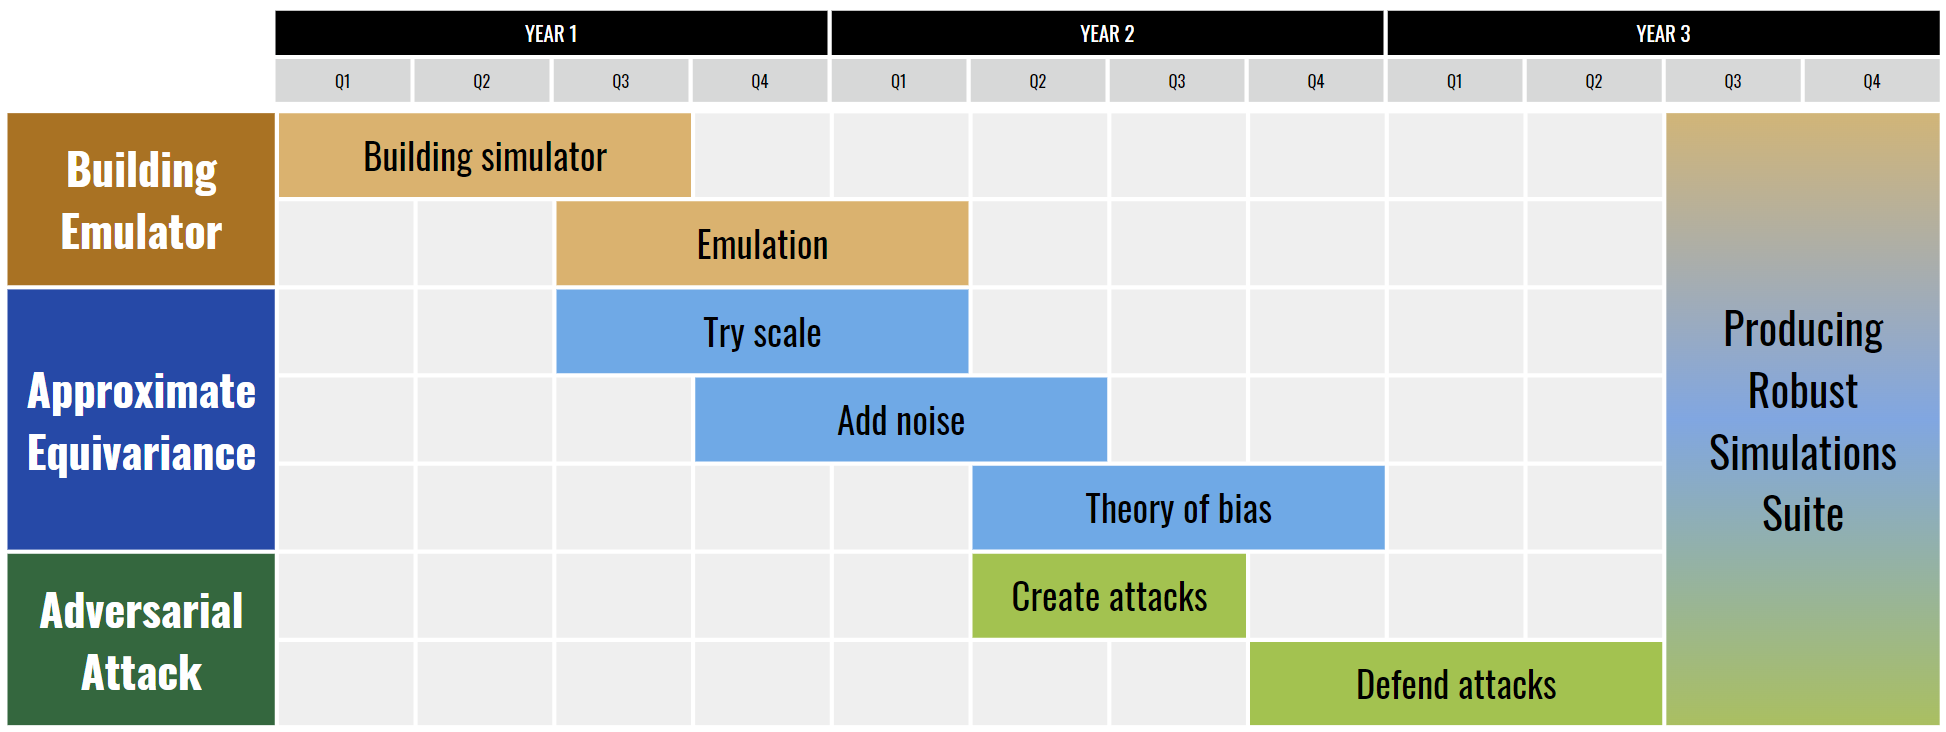
\includegraphics[width=0.9\linewidth]{figures/ONR_gnatt_chart.png}
    \caption{Caption}
    \label{fig:timeline}
\end{figure}

\kw{We should mention we are going to deliver robust ML ocean models that are fast and robust, along with results in understanding the robustness of ML}

\section{\raggedright Budget summmary, timeline, management plan}

There are two budgets for this proposal, one in the NYU Department of Physics, and one in the JHU Applied Mathematics and Statistics Department.
The NYU budget will support two 12-month graduate student researchers, one in the Physics Department and one at Courant Institute.
The JHU budget will give partial salary to research professor Kaze Wong, and support a part-time undergraduate researcher.
In addition, the three PIs will receive a small amount of summer salary support.

Regular meetings at NYU, regular meetings at JHU, and joint meetings at both places occasionally.


\bibliographystyle{IEEEtran}
\bibliography{emulator}

\end{document}